\section{Coinbase Exchange}

To simulate a real world security, I use high frequency LOB data of cryptocurrency securities from Coinbase Pro. Coinbase Pro (formerly known as Global Digital Asset Exchange or GDAX) is the advanced trading platform of the Coinbase, which is an exchange founded in 2012 that brokers trades of many cryptocurrencies, as well as fiat-currency to cryptocurrency exchanges. Major cryptocurrencies that are traded on Coinbase Pro include Bitcoin, Bitcoin Cash, Ethereum, Ethereum Classic, Litecoin, while fiat-currencies are typically the USD or Euro. As of November 2018, Coinbase Pro has a total daily trading volume of about \$150 million (\cite{L1}). I choose to use Coinbase Pro since it has readily accessible real-time LOB data that is freely available to developers from its API. It also features relatively liquid securities with large trading volumes. 

Although the LOB dynamics of the securities that I model in this paper may not entirely reflect those of securities from other exchanges such as stocks, futures, etc., I hope that the methodology in this paper is easily adaptable given LOB data of any type of security. The trading rules of Coinbase Pro are representative of most exchanges. Coinbase Pro allows limit and market orders with time priority. It also allows stop orders, which is an order to place a limit or market order when the price of the security reaches a specified price. Coinbase Pro also differentiates between “maker” and “taker” orders. Taker orders are orders that fill immediately (such as market orders) and maker orders are orders that do not fill immediately and thus populate the LOB (such as limit orders). The fee structure, which is up to 0.3\% for taker orders depending on the volume and 0\% for maker orders encourages market making and therefore increases liquidity of the market. There are also rules to prevent self-trade, which is when the same trader acts as both the maker and taker for a trade. In addition, there are minimum and maximum orders for each security. Full trading rules for Coinbase Pro can be found on its website (\cite{L2}).

\section{Data Collection}
Data is collected through the Coinbase Pro API using a Python library called CoPrA, which is an asynchronous web socket client (\cite{L3}). Specifically, I use Coinbase Pro's "level2" channel, which provides me with a snapshot of the LOB. It also provides updates at every position of the LOB whenever an order happens. See listing \ref{data-collection-code} for the code written. Using these updates, I can maintain an internal LOB to use for data analysis. I have collected data for several days in the months of December and January of all the updates on the LOB of Ethereum Classic using USD (ETC-USD ticker), which has around \$2 million volume of trades each day. For example, the data for December 30, 2018 is shown below, which contained about 330000 updates, where the initial LOB is shown  in Figure \ref{fig:12_30_18_LOB_pic}. The 10 best bids and asks are shown where the vast majority of updates are made, but the LOB also features prices closer to the reference price.

\begin{figure}[t]
\begin{center}
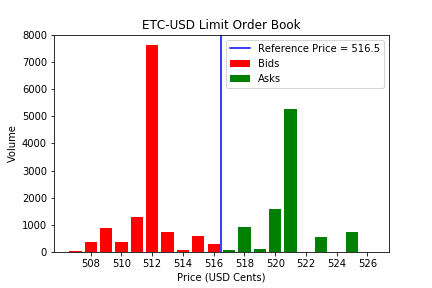
\includegraphics[width=0.8\textwidth]{Figures/12_30_18_LOB.png}
\caption{LOB Sample}
\label{fig:12_30_18_LOB_pic}
\end{center}
\end{figure}

This LOB is typical for ETC-USD, with most of the positions near the reference price filled. The bid and ask sides are relatively balanced, meaning that the reference price is stable. This is not always the case, as the bid or ask side could have significantly more volume when the price shifts. The first 20 updates are also shown in Figure \ref{fig:12_30_18_Updates}.

\begin{figure}[t]
\begin{center}
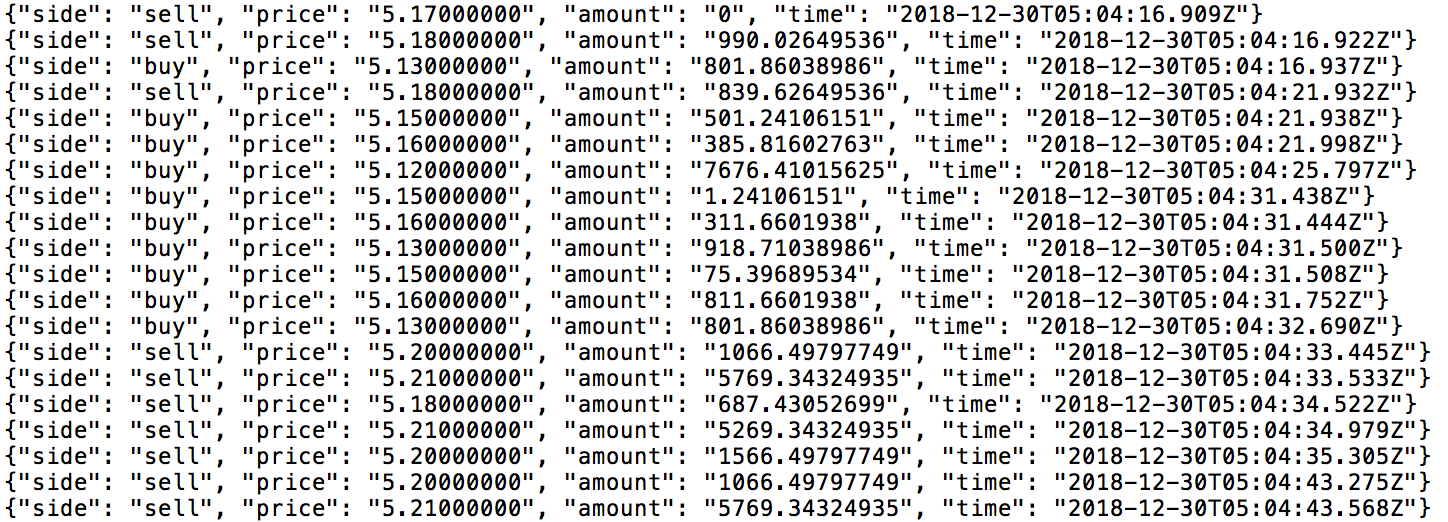
\includegraphics[width=0.8\textwidth]{Figures/12_30_18_Updates.png}
\caption{LOB Updates}
\label{fig:12_30_18_Updates}
\end{center}
\end{figure}

As can be seen, the majority of the updates are given to the nearest millisecond and the majority of the updates occur near the reference price and updates are given to the nearest millisecond.